\documentclass[11pt,parskip]{beamer}
% % % % % PACKAGES

%General Packages
							
\usepackage{amsfonts}												%Mathematics fonts
\usepackage{mathtools}												%General mathematics symbols
\usepackage{amsmath}
\usepackage{stmaryrd}												%Extra math symbols
\usepackage{amssymb}												%More symbols
\usepackage{extarrows}												%Extendible arrows
\usepackage{dsfont} 												%Identity matrix symbol
\usepackage{mathrsfs}												%To get mathscr
\usepackage{relsize}												%Scaling symbols with reference to pre-existing symbols
\usepackage{accents}												%Accents on math symbols
\usepackage[T1]{fontenc}											%Accents output improvement
\usepackage[utf8]{inputenc}										%Accents input improvement
\usepackage[english]{babel}
\usepackage{subcaption} 											%Subfigures etc
\usepackage{cancel} 												%Striking through things
\usepackage{setspace}												%line spacing
\usepackage{enumerate} 												%Numbered lists
\usepackage{booktabs}

%Pictures & TikZ Packages

\usepackage{graphicx}												%Pictures	
\usepackage{epstopdf}												%Converts .eps to .pdf files
\usepackage{tikz}													%TikZ Drawings
\usetikzlibrary{3d,patterns,arrows,bending,arrows.meta,				%TikZ Libraries
	shapes.geometric,knots,intersections,
	decorations.markings,decorations.pathmorphing,
	decorations.pathreplacing}										
\usepackage{tikz-cd}												%Commutative Diagrams
\usepackage{xcolor}

%Mathematics Packages

\usepackage{amsthm}													%Theorems etc



\usepackage[
backend=biber,
doi=false,
eprint=false,
url=false,
isbn=false,
natbib=true,
style=numeric,
citestyle=numeric,
sorting=none,
firstinits=true
]{biblatex}
\addbibresource{thesis-references.bib}

\appto{\bibsetup}{\raggedright}
\addbibresource{thesis-references.bib}
\renewbibmacro{in:}{%
	\ifentrytype{article}{}{\printtext{\bibstring{in}\intitlepunct}}}

\AtEveryBibitem{\clearfield{pagetotal}\clearfield{series}\clearfield{number}}
\AtEveryBibitem{%
	\ifentrytype{article}
	{}
	{\clearfield{volume}}}

% % % % % CUSTOM COMMANDS

%Derivatives/Differentials

\let\underdot=\d
\newcommand{\od}[2]{\frac{\mathrm{d} #1}{\mathrm{d} #2}}
\newcommand{\odd}[2]{\frac{\mathrm{d}^2 #1}{\mathrm{d} #2^2}}
\newcommand{\p}{\partial}
\newcommand{\pd}[2]{\frac{\partial #1}{\partial #2}}
\newcommand{\pdd}[2]{\frac{\partial^2 #1}{\partial #2^2}}
\newcommand{\fd}[2]{\frac{\delta #1}{\delta #2}}
\renewcommand{\d}{\mathrm{d}}
\newcommand{\dif}{D}


%Common Sets/Spaces

\newcommand{\RP}{\mathbb{R}\mathrm{P}}
\newcommand{\CP}{\mathbb{C}\mathrm{P}}
\newcommand{\HP}{\mathbb{H}\mathrm{P}}
\renewcommand{\P}{\mathbb{P}}
\newcommand{\N}{\mathbb{N}}
\newcommand{\Z}{\mathbb{Z}}
\newcommand{\Q}{\mathbb{Q}}
\newcommand{\R}{\mathbb{R}}
\newcommand{\C}{\mathbb{C}}
\renewcommand{\H}{\mathbb{H}}
\renewcommand{\O}{\mathbb{O}}

%Math-operators



\renewcommand{\Im}{\operatorname{Im}}
\renewcommand{\Re}{\operatorname{Re}}

\DeclareMathOperator{\Graph}{graph}
\DeclareMathOperator{\Gr}{Gr}

\DeclareMathOperator{\im}{im}
\DeclareMathOperator{\rank}{rank}
\DeclareMathOperator{\ord}{ord}
\DeclareMathOperator{\tr}{tr}
\DeclareMathOperator{\incl}{incl}
\DeclareMathOperator{\pr}{proj}
\DeclareMathOperator{\diag}{diag}
\DeclareMathOperator{\Span}{span}
\DeclareMathOperator{\codim}{codim}

\DeclareMathOperator{\Hom}{Hom}
\DeclareMathOperator{\End}{End}
\DeclareMathOperator{\Aut}{Aut}
\DeclareMathOperator{\coker}{coker}
\DeclareMathOperator{\Stab}{Stab}
\DeclareMathOperator{\Diff}{Diff}
\DeclareMathOperator{\Bs}{Bs}
\DeclareMathOperator{\id}{id}
\DeclareMathOperator{\Mat}{Mat}
\newcommand{\Unit}{\mathds{1}}

\DeclareMathOperator{\td}{td}
\DeclareMathOperator{\ch}{ch}
\DeclareMathOperator{\Spin}{Spin}
\newcommand{\Spinc}{\Spin^c}

\DeclareMathOperator{\Ad}{Ad}
\DeclareMathOperator{\ad}{ad}

\DeclareMathOperator{\supp}{supp}
\DeclareMathOperator{\interior}{int}
\DeclareMathOperator{\vol}{vol}

\DeclareMathOperator{\sgn}{sgn}

\DeclareMathOperator{\Tor}{Tor}
\DeclareMathOperator{\Ext}{Ext}
\DeclareMathOperator*{\free}{\scalerel*{\ast}{\scaleobj{1}{\sum}}}

\newcommand{\trans}{\mathrel{\text{\tpitchfork}}}
\makeatletter
\newcommand{\tpitchfork}{%
	\vbox{
		\baselineskip\z@skip
		\lineskip-.52ex
		\lineskiplimit\maxdimen
		\m@th
		\ialign{##\crcr\hidewidth\smash{$-$}\hidewidth\crcr$\pitchfork$\crcr}
	}%
}
\makeatother

%Other

%\newcommand{\action}{\curvearrowright}
%\newcommand{\rightaction}{\curvearrowleft}

\newcommand{\ubar}[1]{\underaccent{\bar}{#1}}
\def\mathunderline#1#2{\color{#1}\underline{{\color{black}#2}}\color{black}}

\newcommand{\abs}[1]{\left\lvert #1 \right\rvert}
\newcommand{\norm}[1]{\left\lVert #1 \right\rVert}
\newcommand{\expvalue}[1]{\left\langle #1 \right\rangle}

\setlength{\parindent}{0pt}

\newcommand{\mf}[1]{\mathfrak{#1}}
\newcommand{\mc}[1]{\mathcal{#1}}
\newcommand{\ms}[1]{\mathscr{#1}}

\newcommand{\bdy}{\partial}
\newcommand{\pt}{\mathrm{pt}}
\DeclareMathOperator{\Bl}{Bl}


%Theorem Styles

\newtheoremstyle{mythm}% name of the style to be used
{}% measure of space to leave above the theorem. E.g.: 3pt
{}% measure of space to leave below the theorem. E.g.: 3pt
{\slshape}% name of font to use in the body of the theorem
{}% measure of space to indent
{\bfseries\sffamily}% name of head font
{.}% punctuation between head and body
{ }% space after theorem head; " " = normal interword space
{}% Manually specify head
\newtheoremstyle{mydef}% name of the style to be used
{}% measure of space to leave above the theorem. E.g.: 3pt
{}% measure of space to leave below the theorem. E.g.: 3pt
{}% name of font to use in the body of the theorem
{}% measure of space to indent
{\bfseries\sffamily}% name of head font
{.}% punctuation between head and body
{ }% space after theorem head; " " = normal interword space
{}% Manually specify head

\theoremstyle{mythm}
\newtheorem{thm}{Theorem}[section]
\newtheorem{prop}[thm]{Proposition}
\newtheorem{cor}[thm]{Corollary}
\newtheorem{lem}[thm]{Lemma}
\theoremstyle{mydef}
\newtheorem{mydef}[thm]{Definition}
\newtheorem{rem}[thm]{Remark}
\newtheorem{ex}[thm]{Example}
\newtheorem{exer}{Exercise}[subsection]
\newenvironment{myproof}[1][\proofname]{
	\proof[\sffamily\upshape#1]
}{\endproof}

\newcommand{\proofclear}{\hfill \qedsymbol}

% % % % % MISCELLANEOUS STUFF

\setbeamertemplate{bibliography item}{\insertbiblabel}

\newcommand\numberthis{\stepcounter{equation}\tag{\theequation}}


\newenvironment{numberedlist}{\begin{enumerate}[\upshape(i)]}{\end{enumerate}}
\newenvironment{letteredlist}{\begin{enumerate}[\upshape a)]}{\end{enumerate}}

\usetheme{CambridgeUS}
\usecolortheme{rose}
\title[]{Invariant Geometric Structures and \\ Chern numbers of  $G_2$ Flag Manifolds}
\author[]{Dani\"el Thung\\[0.5cm]}
\institute[]{{\small LMU M\"unchen}\\[0.25cm]}
\date{{\footnotesize September 28, 2017}}

\begin{document}

\begin{frame}[plain]
\maketitle
\end{frame}

\begin{frame}{Outline}
	\begin{enumerate}
		\item Generalized flag manifolds
		\bigskip
		\item $G_2$ and its flag manifolds
		\bigskip
		\item The twistor space
		\bigskip
		\item The quadric
	\end{enumerate}
\end{frame}

\begin{frame}{Generalized flag manifolds}
	\begin{mydef}
		A \emph{flag} is a strictly increasing sequence 
		\begin{equation*}
			\{0\}=V_0\subset V_1 \subset V_2 \subset \dots \subset V_k=V \qquad \qquad k\leq n
		\end{equation*}
		of subspaces of an $n$-dimensional vector space $V$ (e.g.~$\C^n$). Set $d_i=\dim V_i$; then $(d_1,\dots, d_{k-1})$ is the signature of the flag. If $d_i=i$, we call the flag \emph{complete} and otherwise we have a \emph{partial} flag. 
	\end{mydef}	
\end{frame}
\begin{frame}{Generalized flag manifolds}
	\begin{ex}[Flag manifolds of flags in $\C^n$]
		\begin{letteredlist}
			\item The Grassmannian of $k$-planes parametrizes flags of signature $(k)$:
			\begin{equation*}
				\Gr_k(\C^n)\cong \frac{U(n)}{U(k)\times U(n-k)} 
				\cong \frac{SU(n)}{S(U(k)\times U(n-k))}
			\end{equation*}\pause
			\item The \emph{complete} flag manifold is $U(n)/T^n\cong SU(n)/T^{n-1}$.
		\end{letteredlist}
	\end{ex}
\end{frame}
\begin{frame}{Generalized flag manifolds}
	In general, any \emph{flag manifold} of flags in $\C^n$ is of the form
	\begin{equation*}
		\frac{SU(n)}{S(U(r_1)\times\dots U(r_k))}
	\end{equation*}
	where $\{r_1,\dots,r_k\}$ is an ordered partition of $n$. The isotropy subgroup is the centralizer of a torus $T^{k-1}\subset SU(n)$.\pause
	\bigskip
	
	This naturally generalizes to:

	\begin{mydef}
		A \emph{generalized flag manifold} is a homogeneous space of the form $G/C(T)$, where $G$ is a compact, connected and semisimple Lie group, and $C(T)$ is the centralizer of a torus $T\subset G$.
	\end{mydef}
\end{frame}

\begin{frame}{Generalized flag manifolds}
	Generalized flag manifolds carry interesting invariant complex-geometric structures:\pause
	\bigskip
	
	\begin{thm}[Borel~\cite{Bor1953}, Koszul~\cite{Kos1955}, Matsushima~\cite{Mat1957}]
		Every generalized flag manifold admits an invariant complex structure and a unique (up to scaling) compatible invariant K\"ahler-Einstein metric, which has positive scalar curvature. Conversely, any compact, simply connected homogeneous space that admits an invariant K\"ahler metric is isomorphic to a generalized flag manifold.
	\end{thm}\pause
	\bigskip
	
	Furthermore, certain examples are known to carry multiple invariant almost complex structures with distinct Chern numbers (cf. Borel \& Hirzebruch~\cite{BH1958a}).
\end{frame}

\begin{frame}{Generalized flag manifolds}
	Invariant structures are traditionally studied by means of Lie theory, obscuring the geometric meaning of many results.\pause 
	\bigskip
	
	\begin{alertblock}{Objective}
		Study generalized flag manifolds \emph{geometrically} and give a concrete interpretation of their invariant geometric structures.
	\end{alertblock}\pause
	\bigskip
	
	This program was carried out for $SU(n)/S(U(n-2)\times U(1)\times U(1))$ by Kotschick \& Terzi\'c~\cite{KT2009}.
\end{frame}

\begin{frame}[fragile]{$G_2$ and its flag manifolds}
	The exceptional Lie group $G_2$ is the automorphism group of the octonions $\O$. Its generalized flag manifolds fit into the following diagram: \pause
	\begin{figure}\centering
		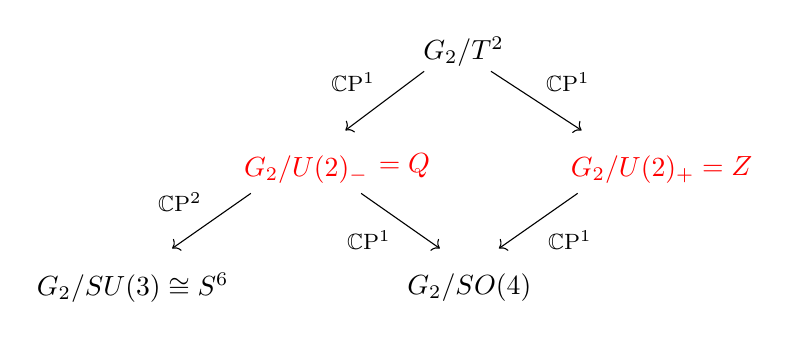
\begin{tikzpicture}
			\draw (3,3) node{$G_2/T^2$};\pause
			\draw (1,1.5) node{\color{red}{$G_2/U(2)_-$}};
			\draw[->] (2.5,2.75) -- (1.5,2)
				node[pos=0.5, anchor=south east]{\footnotesize{$\CP^1$}};\pause
			\draw (-1.2,0) node{$G_2/SU(3)\cong S^6$};
			\draw[->] (0.3,1.2) -- (-0.7,0.5)
				node[pos=0.5, anchor=south east]{\footnotesize{$\CP^2$}};\pause
			\draw[->] (3.35,2.75) -- (4.5,2)
				node[pos=0.5, anchor=south west]{\footnotesize{$\CP^1$}};
			\draw (5.15,1.5) node{\color{red}{$G_2/U(2)_+$}};\pause
			\draw[->] (1.7,1.2) -- (2.7,0.5)
				node[pos=0.5, anchor=north east]{\footnotesize{$\CP^1$}};
			\draw[->] (4.45,1.2) -- (3.45,0.5)
				node[pos=0.5, anchor=north west]{\footnotesize{$\CP^1$}};
			\draw (3.075,0) node{$G_2/SO(4)$};\pause
			\draw (2.25,1.55) node{\color{red}{$=Q$}};
			\draw (6.35,1.55) node{\color{red}{$=Z$}};
		\end{tikzpicture}
	\end{figure}
\end{frame}

\begin{frame}{The twistor space}
	$\pi:Z\to G_2/SO(4)$ exhibits $Z$ as the \emph{twistor space} over $G_2/SO(4)$, which is a quaternionic K\"ahler manifold. \pause
	
	\bigskip
	
	\begin{mydef}
		A quaternionic K\"ahler (QK) manifold is an (oriented) Riemannian manifold of dimension $4n$, $n\geq 2$, whose holonomy group is contained in the subgroup $Sp(n)\cdot Sp(1)$ of $SO(4n)$.
	\end{mydef}\pause

	\bigskip

	Reduced holonomy implies curvature restrictions: QK manifolds are Einstein. 
\end{frame}

\begin{frame}{The twistor space}
	Any QK manifold $M$ carries a rank 3 subbundle $E$ of $\End TM$, locally spanned by a quaternionic triple $\{I,J,IJ=K\}$.\pause
	
	\medskip
	
	\begin{mydef}[Salamon~\cite{Sal1982}]
		The total space $S(E)$ of the sphere bundle of $E$ is called the \emph{twistor space} over $M$.
	\end{mydef}\pause

	\medskip
	
	A point $z=\alpha I+\beta J+ \gamma K \in S(E)$ corresponds to an orthogonal complex structure on $T_{\pi(z)}M$.
\end{frame}

\begin{frame}{The twistor space}
	\begin{thm}[Salamon~\cite{Sal1982}, B\'erard-Bergery~\cite{Bes2008}]
		\begin{numberedlist}
			\item $S(E)$ admits a natural (integrable) complex structure.
			\item If $M$ has positive scalar curvature, then $S(E)$ admits a K\"ahler-Einstein metric with positive scalar curvature.
		\end{numberedlist}
	\end{thm}\pause
	\medskip 
	
	\begin{myproof}[Proof of (i)]
		$TS(E)\cong \mc V\oplus \mc H$, where $\mc H_z\cong T_{\pi(z)}M$; we define a complex structure $J=J_v\oplus J_h$ as follows: $J_v=J^\text{std}_{\CP^1}$, while $z\in S(E)$ \emph{is} the image of $J_h$ under the identification $\mc H_z\cong T_{\pi(z)}M$. The Nijenhuis tensor is explicitly shown to vanish.
	\end{myproof}
\end{frame}

\begin{frame}{The twistor space: Rigidity of the K\"ahler structure}
	Using the Gysin sequence we determine the cohomology ring and Pontrya\-gin classes of $Z=G_2/U(2)_+$. Additively, the cohomology is that of $\CP^5$, but the ring structure is different.\pause
	
	\bigskip 
	
	\begin{thm}
		Let $X$ be a K\"ahler manifold. If it is homeomorphic to $Z$, then it is biholomorphic to $Z$
	\end{thm}\pause
	
	\bigskip
	
	This is the exact analog of rigidity results of Hirzebruch \& Kodaira~\cite{HK1957} (and Yau~\cite{Yau1977}) for $\CP^n$, and Brieskorn~\cite{Bri1964} for $Q_n$ ($n\geq 3$).
\end{frame}



\begin{frame}{The twistor space: Rigidity of the K\"ahler structure}
	\begin{myproof}[Sketch of Proof]
		We have $c_1(X)=d\cdot g_2$, where $g_2$ is the positive generator of $H^2(X;\Z)$. The Chern number $c_1c_4[X]$ is fixed by $h^{p,q}(X)=$ $h^{p,q}(\CP^5)$, hence $c_1c_4[X]=90$. Thus, $d$ divides $90$. Every possibility except $d=3$ is ruled out case-by-case, using the Pontryagin classes as well as the Todd genus, which is also determined by the Hodge numbers.\pause
	
		\bigskip
		
		Once $c_1(X)$ is fixed, Mukai's classification of Fano manifolds of coindex $3$ finishes the proof.	
	\end{myproof}
\end{frame}

\begin{frame}{The twistor space: Invariant almost complex structures}
	\pause
	The second invariant almost complex structure is obtained by ``flipping the fiber'': $J'=(-J_v)\oplus J_h$. The Chern numbers are (compare GNO~\cite{GNO2017}):\pause
	\begin{prop}
		The Chern numbers of the two invariant almost complex structures on the twistor space are:\vspace{-0.5cm}
		\begin{table}[ht!]\centering
			\begin{tabular}{lll} \toprule
				Chern Number& $Z$		& $N$ \\ \midrule
				$c_5$ 		& $6$		& $6$ \\
				$c_1^5$ 	& $4374$	& $-18$\\
				$c_1^3c_2$	& $2106$	& $-6$\\
				$c_1^2c_3$	& $594$		& $18$\\
				$c_1c_4$	& $90$		& $18$\\
				$c_1c_2^2$	& $1014$	& $-2$\\
				$c_2c_3$	& $286$		& $6$\\ \bottomrule
			\end{tabular}
		\end{table}
	\end{prop}
\end{frame}

\begin{frame}{Reminder: $G_2$ flag manifolds}
	\begin{figure}\centering
		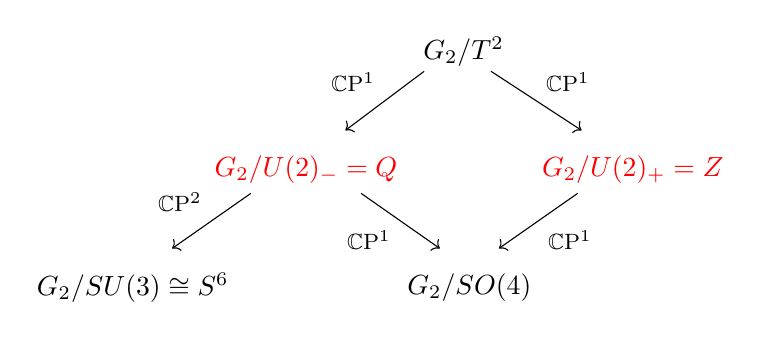
\begin{tikzpicture}
		\draw (-1.2,0) node{$G_2/SU(3)\cong S^6$};
		\draw (1,1.5) node{\color{red}{$G_2/U(2)_-=Q$}};
		\draw[->] (0.3,1.2) -- (-0.7,0.5) 
		node[pos=0.5, anchor=south east]{\footnotesize{$\CP^2$}};
		\draw (3,3) node{$G_2/T^2$};
		\draw[->] (2.5,2.75) -- (1.5,2)
		node[pos=0.5, anchor=south east]{\footnotesize{$\CP^1$}};
		\draw[->] (3.35,2.75) -- (4.5,2)
		node[pos=0.5, anchor=south west]{\footnotesize{$\CP^1$}};
		\draw (5.15,1.5) node{\color{red}{$G_2/U(2)_+=Z$}};
		\draw[->] (1.7,1.2) -- (2.7,0.5)
		node[pos=0.5, anchor=north east]{\footnotesize{$\CP^1$}};
		\draw[->] (4.45,1.2) -- (3.45,0.5)
		node[pos=0.5, anchor=north west]{\footnotesize{$\CP^1$}};
		\draw (3.075,0) node{$G_2/SO(4)$};
		\end{tikzpicture}
	\end{figure}
\end{frame}

\begin{frame}{The quadric}
	$G_2/U(2)_-=Q$ is the space of oriented $2$-planes in $\Im\O\cong \R^7$. \pause
	\medskip
	
	Let $\{e_1,e_2\}$ be a positive, orthonormal basis for $P\in Q$ (unique up to $U(1)$-transformation). $\C$-linearly extending the standard inner product $(-,-)_{\R^7}$ to $\C^7$, set $f(z)=(z,z)=\sum z_j^2$. Then $f(e_1+ie_2)=0$.\pause
	\bigskip
	
	This yields a diffeomorphism
	\begin{equation*}
		Q\cong \big\{f(z)=0\big\} \subset \CP^6
	\end{equation*}\pause 
	\medskip
	
	The invariant complex structure and K\"ahler-Einstein metric are inherited from $\CP^6$: The restriction of the Fubini-Study metric is K\"ahler-Einstein, and even $SO(7)$-invariant. 
\end{frame}

\begin{frame}{The quadric: Invariant almost complex structures}
	Equip $S^6$ with its $G_2$-invariant almost complex structure, given by $J_x(v)=x \cdot v$. Then $\P(TS^6)$ inherits an invariant almost complex structure. \pause The identification
	\begin{equation*}
		\text{complex line} \longleftrightarrow \text{oriented 2-plane}
	\end{equation*}
	induces a diffeomorphism $\P(TS^6)\cong Q \cong \P(T^*S^6)$. \pause 
	\bigskip
	
	\begin{rem}
		This shows that a complex structure on $S^6$ gives rise to (at least two) non-standard complex structures on the quadric $Q\subset \CP^6$.
	\end{rem}
\end{frame}

\begin{frame}[fragile]{The quadric: Invariant almost complex structures}
	We have now found three invariant almost complex structures on $G_2/U(2)_-$, out of a total of four.\pause  
	\medskip
	
	The fourth is obtained from the quadric by flipping the fiber over $S^6$. In fact, all four invariant almost complex structures are related by flips: 
	\begin{equation*}
		\begin{tikzcd}[column sep=3.5cm,row sep=1.5cm]
			Q \ar[r,leftrightarrow,"\text{flip }S^6\text{-fibration}"] 
			\ar[d,leftrightarrow,"\text{flip }G_2/SO(4)\text{-fibration}"']
			& X \ar[d,leftrightarrow,"\text{flip }G_2/SO(4)\text{-fibration}"]\\
			\P(T^*S^6) \ar[r,leftrightarrow,"\text{flip }S^6\text{-fibration}"']
			& \P(TS^6)
		\end{tikzcd}
	\end{equation*}
\end{frame}

\begin{frame}{The quadric: Chern numbers}
	The invariant almost complex structures are distinguished by their Chern numbers (compare GNO~\cite{GNO2017}):
	\begin{prop}
		The Chern numbers of the four invariant almost complex structures on $G_2/U(2)_-$ are:\vspace{-0.4cm}
		\begin{table}[ht!]\centering\hspace{1cm}
			\begin{tabular}{lllll} \toprule
				Chern Number& $Q$		& $\P(TS^6)$ 	& $\P(T^*S^6)$	& $X$ \\ \midrule
				$c_5$ 		& $6$ 		& $6$ 			& $6$			& $6$\\
				$c_1^5$ 	& $6250$	& $-486$		& $486$			& $-2$\\
				$c_1^3c_2$	& $2750$ 	& $-162$		& $162$			& $2$\\
				$c_1^2c_3$	& $650$ 	& $18$ 			& $18$			& $2$\\
				$c_1c_4$	& $90$ 		& $18$ 			& $18$			& $-6$\\
				$c_1c_2^2$	& $1210$ 	& $-54$ 		& $54$			& $-2$\\
				$c_2c_3$	& $286$ 	& $6$			& $6$			& $-2$\\ \bottomrule
			\end{tabular}
		\end{table}
	\end{prop}
\end{frame}

\begin{frame}
	
\end{frame}

\begin{frame}[allowframebreaks]\frametitle{References}
\printbibliography
\end{frame}
	
	
\end{document}